%%%%%%%%%%%%%%%%%%%%%%%%%%%%%%%%%%%%%%%%%%%%%%%%%%%%%%%%%%%%%%%%%%%%%%%%%%
% Voltage and flux waveforms of the transformer (Task 3) and the inductor (Task 4), Exercise 06
%%%%%%%%%%%%%%%%%%%%%%%%%%%%%%%%%%%%%%%%%%%%%%%%%%%%%%%%%%%%%%%%%%%%%%%%%%

\begin{figure}[htb]
	\begin{center}
		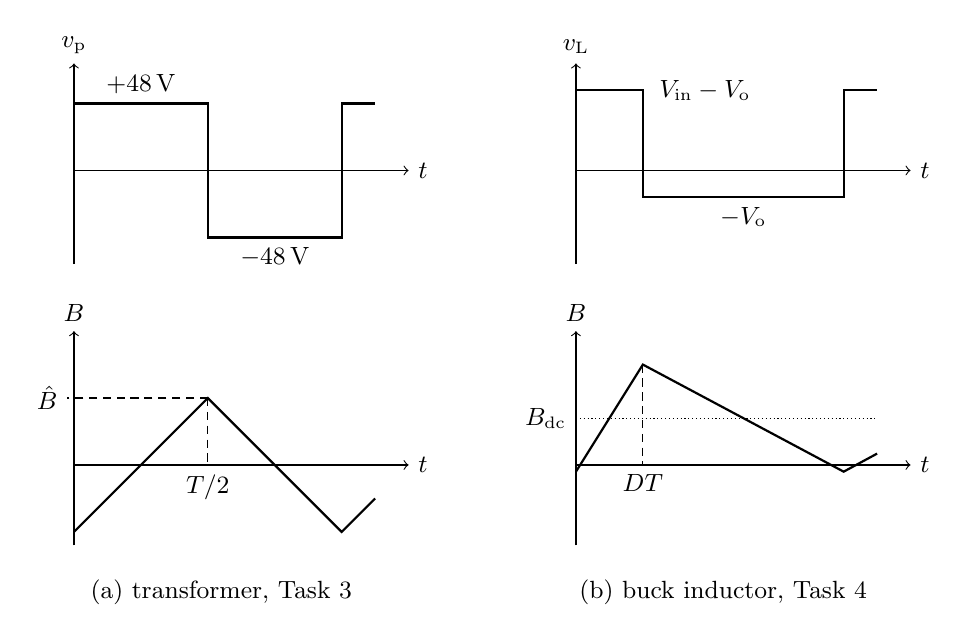
\begin{tikzpicture}[scale=0.85, every node/.style={font=\small}]
			% (a) transformer: square-wave voltage, triangular flux
			\draw[->] (0,0) -- (5.0,0) node[right]{$t$};
			\draw[->] (0,-1.4) -- (0,1.6) node[above]{$v_\mathrm{p}$};
			\draw[thick] (0,1) -- (2,1) -- (2,-1) -- (4,-1) -- (4,1) -- (4.5,1);
			\node[anchor=south] at (1,1) {$+48$\,V};
			\node[anchor=north] at (3,-1) {$-48$\,V};
			\draw[->] (0,-4.4) -- (5.0,-4.4) node[right]{$t$};
			\draw[->] (0,-5.6) -- (0,-2.4) node[above]{$B$};
			\draw[thick] (0,-5.4) -- (2,-3.4) -- (4,-5.4) -- (4.5,-4.9);
			\draw[densely dashed] (2,-3.4) -- (-0.1,-3.4) node[left]{$\hat{B}$};
			\draw[densely dashed] (2,-3.4) -- (2,-4.4) node[below]{$T/2$};
			\node at (2.2,-6.3) {(a) transformer, Task 3};
			% (b) buck inductor: asymmetric voltage, flux with DC component
			\begin{scope}[xshift=7.5cm]
				\draw[->] (0,0) -- (5.0,0) node[right]{$t$};
				\draw[->] (0,-1.4) -- (0,1.6) node[above]{$v_\mathrm{L}$};
				\draw[thick] (0,1.2) -- (1,1.2) -- (1,-0.4) -- (4,-0.4) -- (4,1.2) -- (4.5,1.2);
				\node[anchor=west] at (1.1,1.2) {$V_\mathrm{in}-V_\mathrm{o}$};
				\node[anchor=north] at (2.5,-0.4) {$-V_\mathrm{o}$};
				\draw[->] (0,-4.4) -- (5.0,-4.4) node[right]{$t$};
				\draw[->] (0,-5.6) -- (0,-2.4) node[above]{$B$};
				\draw[thick] (0,-4.5) -- (1,-2.9) -- (4,-4.5) -- (4.5,-4.23);
				\draw[densely dotted] (0,-3.7) -- (4.5,-3.7);
				\node[anchor=east] at (0,-3.7) {$B_\mathrm{dc}$};
				\draw[densely dashed] (1,-2.9) -- (1,-4.4) node[below]{$DT$};
				\node at (2.2,-6.3) {(b) buck inductor, Task 4};
			\end{scope}
		\end{tikzpicture}
	\end{center}
	\caption{Voltage and flux density of the transformer of Task 6.3 and of the inductor of Task 6.4 (not to scale)}
	\label{fig:ex06_waveforms}
\end{figure}
